\chapter{Node Merging} \label{nodemerging}

\section{Node Merging Implementation}
General process of node merging follows like this. Application of rule gives a new graph and it needs to be compared with the existing tree nodes(graphs). If we find that this node exists already, we just add a edge to that node otherwise create a new node. The corresponding code listing can be seen below.

\begin{lstlisting}[language = Java,frame = single]
 for(E rule: rules){
 V newNode = ruleExecutor.execute(node, rule)
 if(newNode != null) {
 /* For all the older nodes in the tree check if it has any match*/
 for(V oldNode:tree.getVertices()){  
        if(nodeComparator.compare(oldNode, newNode)){
	            /* If yes then just add an edge to the existing node */
            Integer edgeId = new Integer(tree.getEdgeCount());
     	    edgeIdToRuleMap.put(edgeId, rule);
    	    tree.addEdge(edgeId, node, oldNode, EdgeType.DIRECTED);
            flag = true;
            break;
        }
    }
 /* If this is a unique graph, create a new node and add it to the tree*/
	   if(!flag){
		    Integer edgeId = new Integer(tree.getEdgeCount()); 
    		edgeIdToRuleMap.put(edgeId, rule);	
	    	tree.addVertex(newNode);
		    tree.addEdge(edgeId, node, newNode, EdgeType.DIRECTED);
        }
    }
}
\end{lstlisting}

\section{Graph Matching}
Two graphs are said to be isomorphic if they have the vertices connected in the same way. Formally, two graphs $G$ and $H$ with graph vertices $V_n =\{1,2,...,n\}$ are said to be isomorphic if there is a permutation $p$ of $V_n$ such that $\{u,v\}$ is in the set of graph
edges $E(G)$ iff $\{p(u),p(v)\}$ is in the set of graph edges $E(H)$.
%Quote: http://mathworld.wolfram.com/IsomorphicGraphs.html

Exact graph matching or graph isomorphism problem is the computational problem of determining whether two finite graphs are isomorphic.graph isomorphism algorithms importance is very high in multiple fields such as electronic design automation, Chemistry and molecular biology etc.

\subsection{Complexity}
Besides its practical importance, the graph isomorphism problem is a curiosity in computational complexity theory as it one of a
very small number of problems belonging to NP, neither known to be solvable in polynomial time nor NP-complete. At the same time, isomorphism
for many special classes of graphs can be solved in polynomial time and in practice, graph isomorphism can often be solved efficiently.
%https://cs.anu.edu.au/people/Brendan.McKay/nauty/PGI/
This is a special case of the subgraph isomorphism problem, which is known to be NP-complete. However Laszlo Babai has claimed that the 
Graph Isomorphism can be solved in quasipolynomial time. Quantities which are exponential in some power of a logarithm are called “quasipolynomial.”
%http://jeremykun.com/2015/11/12/a-quasipolynomial-time-algorithm-for-graph-isomorphism-the-details/

\subsection{Negative checks}
Before going into the algorithm, so called negative checks can be performed to avoid the process of going into the matching algorithm.
\begin{enumerate}
\item \texttt{Vertex number equivalence:} The number of vertices should be equal

\item \texttt{Edge Count equivalence:} The sum of the edges should be equal

\item \texttt{Edge order check:} This is one of the important checks since, when the graphs don't change much, the edge and vertices numbers may not change. Therefore, sorting the edge arrays and 
comparing them will give a good candidates for matching algorithm.
\end{enumerate}

\section{VF2 Algorithm}
Lot of algorithms exists to solve graph isomorphism problem, such as Ullman, nauty, VF2 etc. VF2 algorithm written by Italian scientists was chosen. VFLib developed by same people with the VF2 paper are good point to start writing the custom implementation. 

VFLib defines a single interface (State) that a variety of subgraph isomorphism matchers can implement in order for it to work interchangeably. Understand the VF2 algorithm itself was a big challenge. One of the ways to understand any graph matching algorithm is to understand the commonalities among all of the approaches currently used. Below are the some of the listings of some possibilities. 

\begin{itemize}
\item \texttt{Recursion:} Any implementation typically has a method that calls itself
\item\texttt{State accumulation:} The recursive method gradually building up a map of nodes from source 
graph to target graph, one pair of nodes at a time. Sometime it fails, so it needs to go back to last successful match (backtrack). When it succeeds and needs to report success.
\item \texttt{Mapping:} The implementation typically uses an internal map to keep track of what it's done. So getting getting mapped nodes is easy.
\end{itemize}
 
\begin{figure}
\centerline{
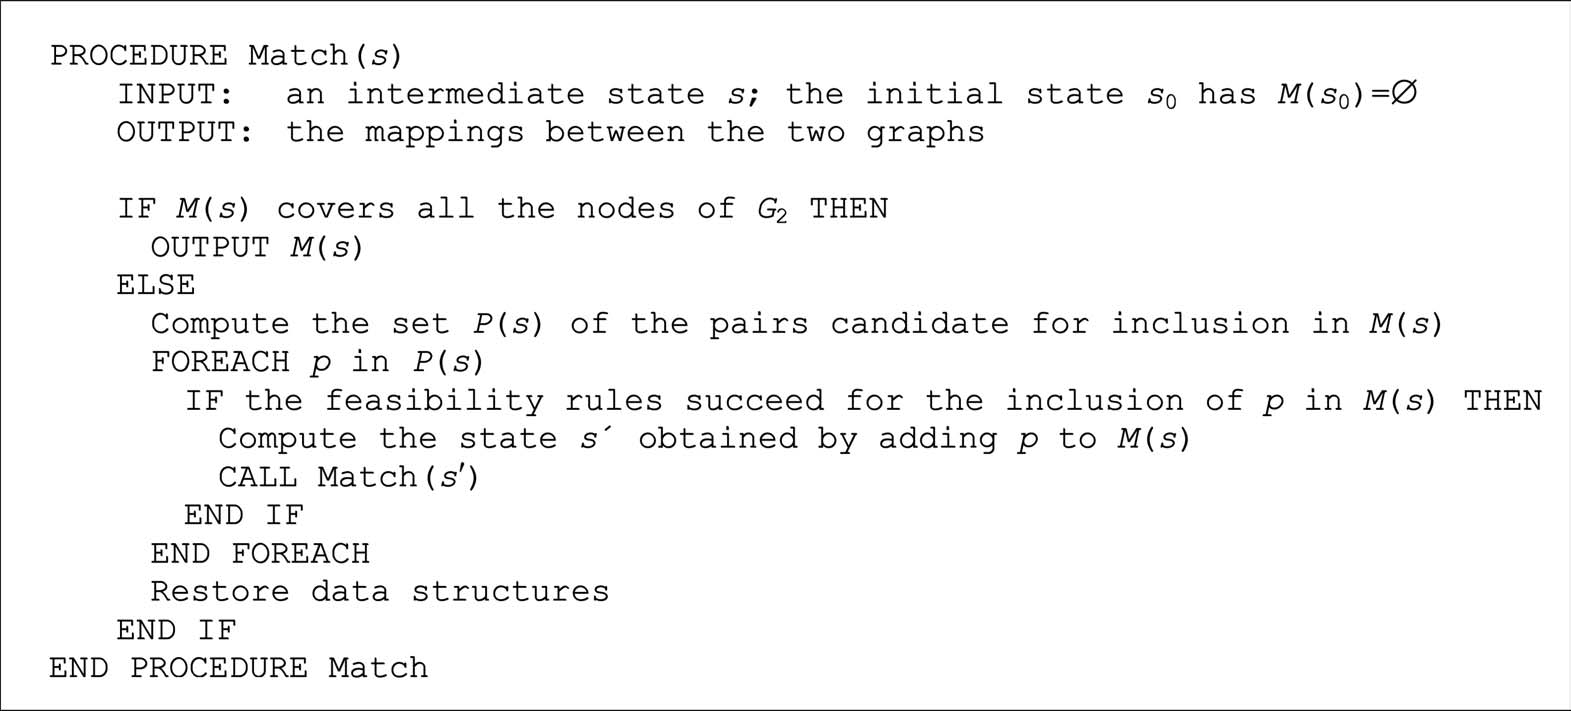
\includegraphics[width=1.0\columnwidth]{figures/vf2_image.png}
}
\caption{VF2 algorithm}
% Quote VF2 paper
\label{vf2}
\end{figure}

The basic idea behind VF2 is that, it tries to find the mapping of vertices between two graphs. 
This process of finding the mapping function can be suitably
described by State Space Representation (SSR). 
%refer vf2 paper
Each state s of the matching process can be associated to a partial
mapping solution M(s), which contains only subset of the complete mapping. A transition from a generic states to a successor state s', represents the addition of a pair of matched nodes to partial mapping associated to s in the SSR. The algorithm explores the search graph in the SSR according to a depth-first search strategy. 

In figure \ref{vf2}, the Match(s) procedure plays the role of recursive function, while s and s' play the dual role of state accumulators and feature comparators. P(s) represents the set of candidates to be added to state s. There are set of feasibility rules can be defined to check the consistency condition. These rules can be both syntactic(depend only on the structure of the graph) and semantic (depends on the attributes of nodes and edges).

\subsection{Implementation}
In the present work basic idea of VF2 is preserved, while lot of modifications were made for the
practical purpose. Hereinafter graph1 is mentioned as source graph and graph2 as target graph.
 
\begin{figure}
\centerline{
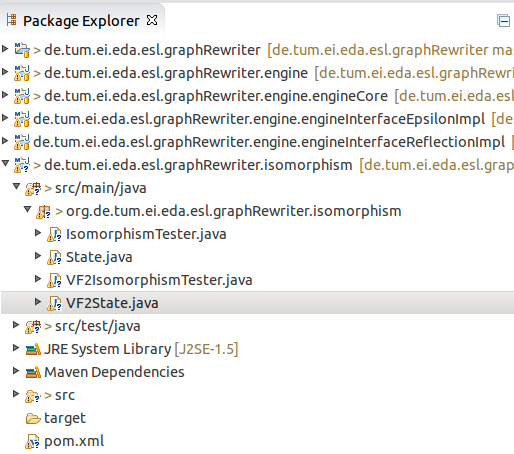
\includegraphics[width=0.6\columnwidth]{figures/folder.png}
}
\caption{folder structure}
\label{folder}
\end{figure}

Figure \ref{folder} shows the VF2 implementation in the current project.
As seen in the figure \ref{folder}
IsomorphismTester.java is an interface which defines a function which will be implemented in VF2IsomorphismTester.java.
\\
\\
\\
\\

\begin{lstlisting}[language = Java,frame = single]
public interface IsomorphismTester {
/*
 * Return true if the graphs are Isomorphic
 */
boolean areIsomorphic(Graph<EObject, EClass> g1, Graph<EObject, EClass> g2);
}
\end{lstlisting}

State.java is an interface, which corresponds to the state s of the VF2 algorithm. VF2State.java implements State interface. 
\\

Before explaining the functions, some of the data structures used are,

\begin{lstlisting}[language = Java,frame = single]
/*possible candidates to add it to state */
private ArrayList<Pair<EObject>> candidates; 
	
private ArrayList<EObject> sourcePath; // Holds matched vertices of source
private ArrayList<EObject> targetPath; // Holds matched vertices of target
	
/*  holds the matched source nodes for each node in the target graph */
public Map<EObject, Set<EObject>> matchedNodeCandidates; 
	
\end{lstlisting}

VF2IsomorphismTester.java defines match procedure along with implementing areIsomorphic() function. 

\begin{lstlisting}[language = Java,frame = single]
boolean areIsomorphic(Graph<EObject,EClass> g1, Graph<EObject, EClass> g2)
{
	State state = new VF2State(g1,g2);
		
	if(!state.checkIndividualMatch()){
		System.out.println("VF2: Individual nodes cann't be matched");
		return false;
	}
	maps.clear();
	match(state);
		
	if(!maps.isEmpty()){
		if(maps.get(0).size() == g1.getVertexCount()) 
		return true;
	}
	return false;
}
\end{lstlisting}


An empty state is created initially, in which the initial candidate is selected as opposed to loading every possible vertex match. A little optimization is carried out to identify a uniques start node(vertex should have only one match in source and target). A further optimization would be to check to see if it has unique neighbors.

\texttt{state.checkIndividualMatch()}, checks if every vertex can be matched between source and target, this is an interesting check since, for each vertex in source we need to have at least one matching vertex in the target.

After this, match function is called. The result is returned based on the number of mapped vertices.

\begin{lstlisting}[language = Java,frame = single]
private boolean match(State s) {
		if(s.isGoal()){
			maps.add(s.getVetexMapping());
			return true;
		}
		if(s.isDead())
			return false;
		
		boolean found = false;		
		while(!found && s.hasNextCandidate()){
			Pair<EObject> candidate = s.nextCandidate();
					
			if(s.isFeasiblePair(candidate)) {
				State nextState = s.nextState(candidate);
						
				found = match(nextState);
			
				if(nextState.backtrack()){			
				}
				else{
					return false;
				}
			}
	}
		return found;
}
\end{lstlisting}

s.isGoal() returns true if all vertices are mapped.\\
s.isDead() returns false when vertex number mismatch happens. 

After the necessary checks, it choses the initial candidate as our start node pair and checks for feasibility of the candidate. And if it is a feasible candidate a next state is created, with the current candidate will be added to map.
And match procedure will be called on the next state. Once we run out of candidates match function returns and checks for backtracking, if it is a successful backtrack matching continues else match will terminate by returning false. \\

\texttt{Feasibility Function Listing}
\begin{lstlisting}[language = Java,frame = single]
public boolean isFeasiblePair(Pair<EObject> match) {
		
		if(map.containsKey(match.getFirst()) 
		|| map.containsValue(match.getSecond()))
		{
			return false;
		}
		
	Set<EObject> matchedNodes = matchedNodeCandidates.get(match.getSecond());
		
		if(!(matchedNodes.contains(match.getFirst())))
				return false;
				
		if(!immNbrMatch(match)){
					return false;
		}
		return true;
		}		
\end{lstlisting}
In original VF2 algorithm there are lot of feasibility rules (semantic and syntactic) are applied before deciding the feasibility. The current graph structure does not lot of checking since we are concerned with node property matching as well. A check is carried out to make sure it is not already mapped and secondly if these candidate data can be matched and lastly if we can map its neighbors. This neighbor checking eliminated lot of potential duplicate candidates and avoid unnecessary backtracking.

\texttt{s.nextState():}
\texttt{s.nextState} returns a new VF2State, by copying all the previous state values and add the current candidate to the state. Additionally it loads the new candidates for matching, which are the combinations of neighbors of previous candidate. 
 
\texttt{Backtrack() Function Listing}
\begin{lstlisting}[language = Java,frame = single]
public boolean backtrack() {
		if(sourcePath.isEmpty() || isGoal()){
			map.clear();
			return true;
		}
		if(isHeadMapped()){
			return true;
		}
	
		EObject last = targetPath.get(targetPath.size()-1);
	
		if(matchedNodeCandidates.get(last).size() == 1){
			return false;
		}
		map.clear();
		
		for(int i = 0; i<sourcePath.size() -1 ; i++)
		{
			map.put(sourcePath.get(i), targetPath.get(i));
		}
		return true;
	}
\end{lstlisting}
Our program spends a lot of time backtracking since, this is essential part to find the appropriate match, but if the necessary checks are not carried out this can increase the time significantly. 
First we check for conditions if its goal or if the mapping hasn't started at all. 
If the head is mapped, which is when we have mapped the candidate and all of its neighbors successfully, then we safely go back to previous step keeping the current mappings. 
If these conditions fail, then we remove the last mapped candidate and continue the process.

There is one more important check needs to be carried out to avoid backtracking to a great deal. Since we have matchedNodeCandidates(map of all vertices matches between source and target) which can be used effectively to determine if removal of the last matched candidate and continuing would yield the result. To remove the last successful match, there should be different vertices to match for these candidate vertices. If we don't have any then we need to stop backtracking, since there can be no vertex which can be mapped to candidate vertices.

\section{Results}
The most of the comparisons were eliminated by negative checks and individual node matching step. For graph which has 315 nodes the time taken for successful match is 17 seconds and for unsuccessful match is 12.5 seconds. This is generally good result considering the setup time.

Figure \ref{result} shows the resulting graph obtained by node merge. 
\begin{figure}
 \centerline{
 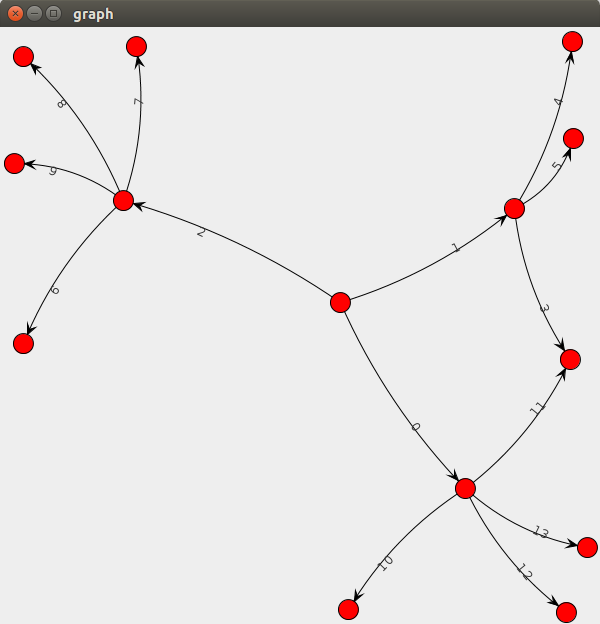
\includegraphics[width=1.0\columnwidth]{figures/result.png}
 }
 \caption{Resultant graph after node merge}
 % Quote VF2 paper
 \label{result}
 \end{figure}
 
\section{conclusion}
The implemented algorithm does a good job for exact graph matching, however it can also be used for subgraph isomorphism. The main time consuming part was to understand the algorithm and how it works so that exploiting this for the practical purpose becomes easier.

The main time consuming part is where setting up the array of individual vertex map. Overall it is efficient for practical usage purpose where it exploits the graphs characteristics, however further improvements can be carried out, like making the interfaces to work on generic data structures which will be part of future work and with little changes it can be extended for subgraph isomorphism as well.  
